\documentclass[11pt,letterpaper]{article}

\newenvironment{proof}{\noindent{\bf Proof:}}{\qed\bigskip}

\newtheorem{theorem}{Theorem}
\newtheorem{corollary}{Corollary}
\newtheorem{lemma}{Lemma} 
\newtheorem{claim}{Claim}
\newtheorem{fact}{Fact}
\newtheorem{definition}{Definition}
\newtheorem{assumption}{Assumption}
\newtheorem{observation}{Observation}
\newtheorem{example}{Example}
\newcommand{\qed}{\rule{7pt}{7pt}}

\newcommand{\solution}[4]{
\thispagestyle{plain} 
\newpage
\setcounter{page}{1}
\noindent
\begin{center}
\framebox{ \vbox{
\vspace{4mm}
\vspace{0.2in} 
{\centering \large\mbox{#3}}\\
\vspace{0.1in}
{#1 \hfill {Date: #2}}
}}
\end{center}
\markright{#1}
}

\newenvironment{algorithm}
{\begin{center}
\begin{tabular}{|l|}
\hline
\begin{minipage}{1in}
\begin{tabbing}
\quad\=\qquad\=\qquad\=\qquad\=\qquad\=\qquad\=\qquad\=\kill}
{\end{tabbing}
\end{minipage} \\
\hline
\end{tabular}
\end{center}}

\def\Comment#1{\textsf{\textsl{$\langle\!\langle$#1\/$\rangle\!\rangle$}}}



\usepackage{graphicx, amssymb, amsmath, listings, float, mathtools}
\usepackage{color, url}
\lstset{language = Python}
\lstset{breaklines}
\lstset{extendedchars=false}

\oddsidemargin 0in
\evensidemargin 0in
\textwidth 6.5in
\topmargin -0.6in
\textheight 9.0in

\begin{document}

\solution{\large Jifu Zhao}{\large 09/29/2016}{\bf \Large IE 529 \hspace{0.5cm} 
		Fall 2016 \hspace{0.5cm} Assignment 2}

\section{\large PCA}

Following the procedures of PCA, the mean value is:
$$\vec{m} = [1.87275, \  1.48783, \  1.87275]$$

And the variance is:
$$variance = [2.38297, \  0.234668, \  2.54 \times 10^{-16}]$$

And the corresponding eigenvector is: 
$$eig1 = [-0.6694 \ -0.3220 \  -0.6694]^T$$
$$eig2 = [0.2277 \  -0.9467 \  0.2277]^T$$
$$eig3 = [-0.7071 \  -1.4140 \times 10^{-15} \  0.7071]^T$$


The de-biased dataset and corresponding eigenvectors are plotted in Figure \ref{fig:3d}.

\begin{figure}[H]
\centering
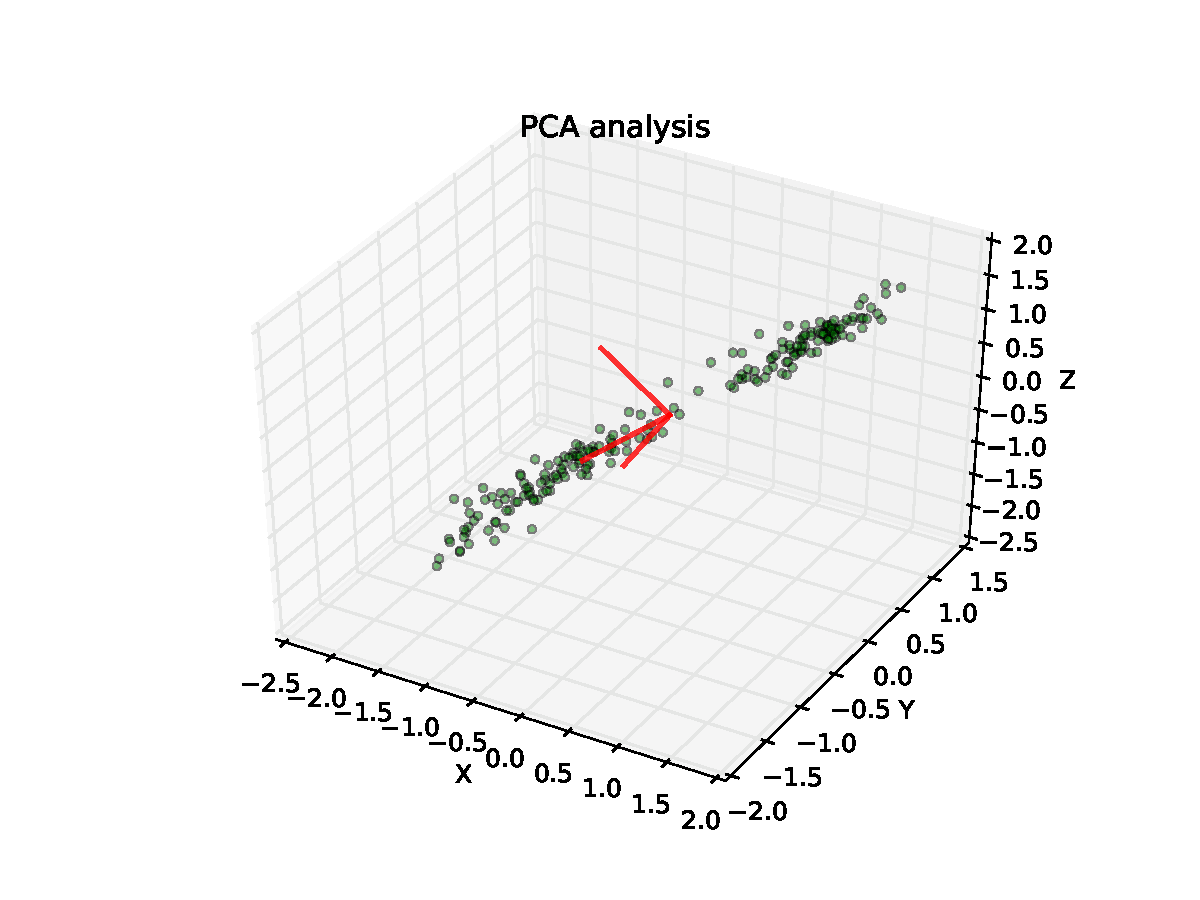
\includegraphics[width=0.9\textwidth]{./figures/3d.pdf}
\caption{\label{fig:3d} PCA eigenvector and scatter plot}
\end{figure}


The original dataset can be projected onto the first two principal components, the result is shown in Figure \ref{fig:projection}.
\begin{figure}[H]
\centering
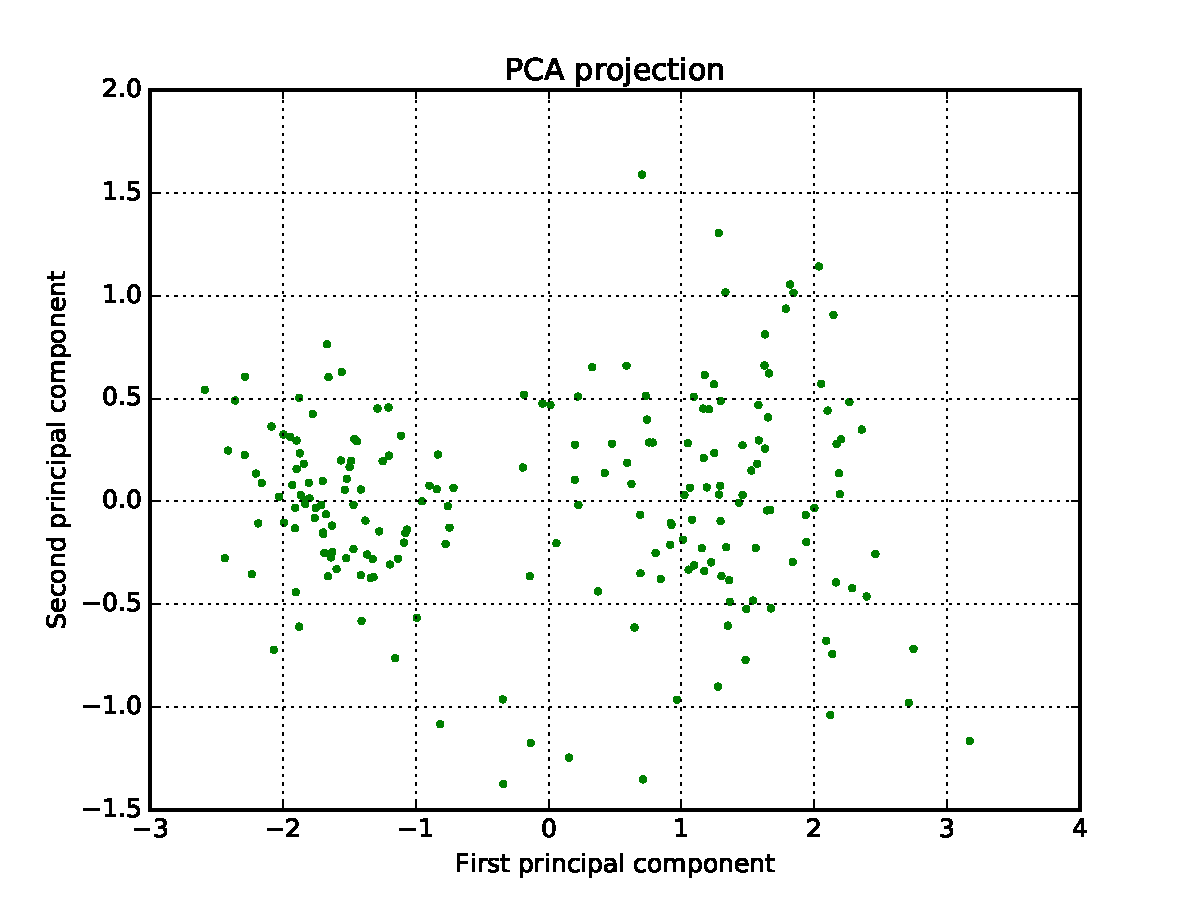
\includegraphics[width=0.9\textwidth]{./figures/projection.pdf}
\caption{\label{fig:projection} PCA Projection}
\end{figure}


\section{\large Discussion}

Currently the PCA is conducted through $$[U, S, V] = SVD(A * A^T)$$

In fact this process can be simplified to: $$[U', S', V'] = SVD(A)$$

Then, we can get that: 
$$U = U'$$
$$S = {S'} ^ 2$$

In this way, this process can be directly performed on the original data, rather than the new data.


\clearpage

%\bibliographystyle{plain}
%\bibliographystyle{unsrt}
%\bibliography{reference.bib}

\end{document}

